\chapter{TIPP: Taxonomic identification and phylogenetic profiling using families of Hidden Markov Models}\label{tipp_chapter}
\index{TIPP@\emph{TIPP}}%

In the previous chapter, I presented SEPP, a method for phylogenetic placement using families of HMMs.  I presented results that show SEPP has improved phylogenetic placement accuracy on evolutionarily divergent datasets.  In this chapter, I will show how SEPP can be used for taxonomic identification, and how SEPP suffers from a high false positive rate under difficult model conditions, such has high rates of sequencing error or sparse taxonomic sampling of the backbone sequences.  I will present TIPP, a modification of SEPP that incorporates statistical support measures to control the precision and sensitivity of classification.  I will show that TIPP classifies more fragments correctly compared to leading taxonomic identification methods, and that TIPP maintains high precision and sensitivity under very difficult conditions.  In addition, experimental results will show that TIPP also improves taxonomic profiling accuracy.  

Section \ref{tipp:motivation} formally describes the taxonomic identification and profiling problem and presents previous work on these problems.  I also show how phylogenetic placement can be applied toward taxonomic identification and profiling and present results on taxonomic identification using SEPP.  In Section \ref{tipp:algorithm}, I describe TIPP, an improved version of SEPP for taxonomic identification and profiling.  In Section \ref{tipp:evaluation}, I describe the simulation study designed to evaluate the performance of TIPP toward taxonomic identification and profiling.  Section \ref{tipp:results}, I present the results comparing TIPP for taxonomic identification and taxonomic profiling.  I show that TIPP outperforms other taxonomic identification methods under difficult conditions and that TIPP generally results in better profiles than leading profiling methods.  Finally, in Section \ref{tipp:conclusion}, I discuss possible ways of improving TIPP, and future studies using TIPP.

\section{Motivation and previous studies}\label{tipp:motivation}
Metagenomic studies of microbial communities commonly generate
millions to hundreds of millions of sequencing reads.  The assignment
of accurate taxonomic labels to these sequences is a critical
component in many analyses, but is
complicated by the fact that the majority of the organisms
found in environmental or host-associated communities cannot be easily
cultured in a laboratory, and an even smaller number have been
sequenced, even partially.  Thus, these commonly encountered organisms
are largely absent from existing databases of known genomes and genes.
Providing taxonomic labels to metagenomic sequences requires
extrapolating the knowledge contained in sequence databases to
previously unseen DNA strings.  Simple similarity-based approaches
(e.g., picking the best database hit as the best `guess' at the
taxonomic label) have been shown to be insufficiently
accurate \cite{closest-blast-hit}, leading to the development of 
new and more sophisticated methods.

Recently developed methods improving
on the simple similarity-based approaches include 
(a) composition-based approaches that rely on
various machine learning techniques 
(Support Vector Machines in
PhyloPythia and PhyloPythiaS \cite{McHardy2007a, Patil2011}, 
Interpolated Markov Models in Phymm 
\cite{Brady2011},
Bayesian models in NBC \cite{Rosen2011}, or neural networks~\cite{SOM2006}) to
classify sequences based on their DNA composition (usually based on
the frequency of short k-mers),
(b)  more sophisticated analyses of
similarity search results (e.g., using least-common-ancestor
aggregation in Megan \cite{Huson2007}, or classifiers built from similarity
search results as done in MetaPhyler \cite{Liu2011d,Liu2011}, 
MetaPhlAn \cite{Segata2012a}, and mOTU \cite{Sunagawa2013}
or protein profiles in Carma \cite{Gerlach2011b}), and
(c) combinations of
multiple approaches (e.g., composition and similarity based approaches
in PhymmBL \cite{Brady2009}).  
Some of these approaches (e.g., most of the
composition-based approaches) can be applied to any DNA sequence,
while others are specific to a reference collection of carefully
selected genes (e.g., MetaPhyler, MetaPhlAn, and mOTU use a collection of
universal or clade-specific marker genes).  These
``marker-gene" methods can
achieve much higher recall than other
approaches~\cite{Liu2011d} for sequences from the marker genes, but 
can only classify a small
fraction of all sequences (namely, those that match the 
selected marker genes). 

Abundance profiling, also called ``phylogenetic profiling", 
seeks to estimate the relative
abundance of the species (or
genera, or families, etc.) within a sequence dataset.
While many methods produce these estimates by characterizing
most (or all) of the sequences in the dataset, marker-based methods
produce these estimates by characterizing only those
sequences that match the marker genes they rely on.
Since the marker genes are supposed to be single
copy and universal, these estimations do not need to
be corrected for the copy number in each genome, or for
missing data. 
However, the restriction to sequences that match the marker genes
has the potential to reduce accuracy since it means only a subset
of the sequences are characterized.

\paragraph{Taxonomic identification through phylogenetic placement.}
One approach toward taxonomic identification is through phylogenetic placement.  The evolutionary relationship between the the query sequence and the backbone sequences can be inferred from the placement location.  For example, in Figure~\ref{tipp:placement}, $Q1$ is placed closest to Species $A1$, and thus, it can be inferred that $Q1$ is more closely related to Species $A1$.  Similarly, $Q2$ is more closely related to Species $A1$ and $A2$ than to Species $B1$ and $B2$.  Thus, one simple technique for identifying a query sequence is to classify it by the LCA of its sibling leaf nodes.  Thus, $Q1$ would be classified as Species $A1$ (its only sibling leaf node is Species $A1$) and $Q2$ would be classified as Genus $A$ (its sibling leaf nodes are Species $A1$ and Species $A2$).  

\begin{figure}[htpb]
\begin{center}
{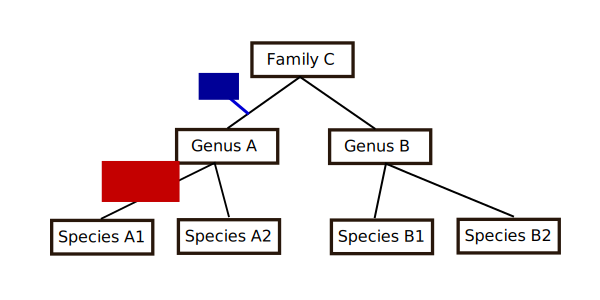
\includegraphics[scale=0.8]{tipp/placement.pdf}}
\end{center}
\caption[Taxonomic classification using phylogenetic placement]{\label{tipp:placement} Taxonomic classification using phylogenetic placement.  The leaf nodes of the rooted backbone tree are labeled with the species name.  Each query sequences is placed onto an edge in the backbone tree and is classified by the LCA its sibling leaf nodes.}
\end{figure}

Using this approach, I compared SEPP and HMMALIGN+pplacer for taxonomic identification under a \emph{leave-species-out} experiment.  Under a leave-species-out experiment, the species of the query sequence is removed from the backbone alignment and tree, simulating the classification of a novel species.  Thus, while the species of the query sequence cannot be correctly identified, the remaining taxonomic lineage (genus, family, etc...) can still be correctly classified.  The fragments were simulated under differring models and rates of sequencing error.  

Figure~\ref{tipp:preliminary_sepp} shows that SEPP is more sensitive than HMMALIGN+pplacer under the hardest model condition (``454\_3''), classifying more fragments correctly, especially at the phylum level.  Both methods tend to classify the large majority of the fragments, leaving very few fragments unclassified.  This results in a very high false positive rate, especially under more difficult conditions.  

To understand why this is the case, it's important to note that pplacer outputs multiple possible locations for the placement of each query sequence.  Each placement has an associated with a likelihood weight ratio.  However, when HMMALIGN+pplacer or SEPP is used for taxonomic classification, only the placement with the likelihood weight ratio is used, ignoring that there may be other placements with almost as high weight.  This was one of the key insights in the development of TIPP.  By taking into account different sources of uncertainty, both in alignment and placement, the false positive rate could be reduced.

\begin{figure}[htpb]
\begin{center}
{\includegraphics[scale=0.4]{{tipp/sepp.species}.pdf}}
\end{center}
\caption[Comparing SEPP and HMMALIGN+pplacer for taxonomic identification]{\label{tipp:preliminary_sepp} Leave-species-out experiments comparing SEPP and HMMALIGN+pplacer taxonomic classification accuracy on the rpsB gene under sequences simulated under different error model conditions.  Fragments were simulated with either Illumina-like or 454-like errors, and with varying rates of error.  Models denoted with a ``1'' have the lowest rates of error, and models with a ``3'' or ``4'' have the highest rates of error.  SEPP is run using a alignment decomposition size of 100 and placing on the entire backbone tree.}
\end{figure}

%Taxon identification methods only classify a
%subset of the fragments (some correctly and some incorrectly), and
%will leave some fragments unclassified at each taxonomic level.
%Therefore, evaluations of taxonomic classification methods
%consider the percent of fragments classified
%at each rank correctly, incorrectly, or unclassified.  

%However, accurate classifications of just the fragments matching
%marker genes is sufficient for many purposes.
%For example, most culture-independent
%studies of microbial communities have relied on the
%analysis of the 16S rRNA gene.
%These studies, generating broad taxonomic profiles of the
%communities being studied, have been the basis for
%many important discoveries in microbial ecology and
%biomedicine  \cite{Turnbaugh2009}. % Alternative: Aagaard2012, Belda-Ferre2012
%In addition, 
%taxon identification methods should accurately label
%sequences already found in public databases, but should also provide accurate
%guesses on the taxonomy of sequences that are only distantly related
%to known sequences.  In fact, identifying novel organisms or taxonomic
%clades is an important focus of recent studies~\cite{eisen} and taxon
%identification software should be able to accurately identify putative
%novel organisms.  


% We have developed TIPP, a new method for taxon
% identification and phylogenetic profiling.
% TIPP is a marker-based method, but can be used to
% characterize any sequence matching any gene for which
% a dense enough sample of full-length sequences are
% available. In this paper, we explore TIPP using the
% Metaphyler's collection of 30 marker genes.

\section{TIPP algorithm}\label{tipp:algorithm}
TIPP uses a statistical pipeline to 
perform taxon identification, as follows.  
In the first step, TIPP uses BLAST \cite{Altschul1990} to 
determine which sequences map to the marker
genes. 
Then, for each bin of sequences matching a given
marker gene, 
TIPP uses a multi-step statistical technique
to taxonomically characterize each sequence.

For a given bin of sequences mapping to a marker
gene, TIPP uses 
SAT\'{e} \cite{Liu2009,Liu2012} to estimate
the multiple sequence alignment and gene tree
on full length sequences for the marker gene.
It then 
uses SEPP \cite{Mirarab2012}, a highly accurate method for phylogenetic placement
that uses a collection of
Hidden Markov Models (HMMs), 
as implemented in HMMER \cite{Eddy1998},
to insert each metagenomic fragment into the alignment.
For each extended alignment produced in this way,
it inserts the fragment into the taxonomy using maximum likelihood
(implemented in pplacer \cite{Matsen2010} or EPA \cite{Berger2011}).
Each placement of the fragment thus provides a taxon identification of
the fragment, and comes with statistical support values for the
estimated
alignment and taxon placement of
the fragment.  To reduce the potential for
false positive classification (and hence improve the
precision of the taxon identification), TIPP allows the user to
specify minimum statistical support levels for both the alignment and
the placement steps.  Given those thresholds, TIPP computes a
set of alignments and placements that suffices to meet the required
statistical support levels, and returns the LCA (least common ancestor) of these
placements as the final placement. The result is a
statistically-based method that can be tuned for precision or recall,
and which has better recall (even for its more
conservative setting) compared to the other marker-based methods.  

If the desired output is the abundance profile of the
sample, then the taxonomic characterizations obtained
for each bin are pooled, and then the distribution is
estimated from the pooled collection.

\paragraph{\bf TIPP's technique for taxonomic identification for
a single marker gene. }
I now describe in greater detail the 
technique used by TIPP to taxonomically identify the
fragments matching a given marker gene.
The input 
is (1) a set $Q$ of fragmentary
sequences from a single gene,
(2) a set $S$ of
full-length sequences for the same gene, and (3)
a taxonomy $T^*$.
%Since metagenomic samples are a mixture of
%reads from different genes and organisms, 
%TIPP can only be used after
%the metagenomic sample is binned into sets, each of which is
%predicted to come
%from the same gene,
%for which we use BLAST.
%\cite{Eddy1998, Altschul1990,  Langmead2009}.

\noindent{\bf Parameter settings for default TIPP.}
I describe the simplest use of TIPP, which is
used for all cases where $n$, the number of full-length sequences
obtained for the marker gene, is not very large (see Section \ref{supp:large_marker}
 for a description of how I modify TIPP when $n$ is very large).  In this simple version of 
TIPP, I do not constrain the portion of the taxonomy
into which the fragment can be inserted.  I also need to set
$m_a$, the maximum alignment size, whether EPA or pplacer is used,
and the statistical support thresholds $s_a$ and
$s_p$ for alignment and placement support, respectively.

I now describe how TIPP performs
a taxonomic identification of a single query sequence $q$:

\noindent{\bf Step 1: Decomposition.}   TIPP uses a SAT\'{e}
alignment and tree on the set $S$ of full
length sequences as the reference alignment $A$ and tree $T$.  I decompose the
reference alignment $A$ and tree $T$ 
into alignments subsets with at most $m_a$ leaves each as follows.  
TIPP finds a centroid edge in $T$ (one that
separates the leaf set into two sets of
approximately equal size), and breaks the tree accordingly into two subtrees.
For each resulting subtree that contains more than $m_a$ leaves, 
TIPP recursively repeats this decomposition.
This produces a partition of $S$  into subsets $S_1, S_2, \ldots, S_k$,
each of size at most $m_a$.

\noindent{\bf Step 2: Compute Extended Alignment. }  
For a given alignment subset of sequences $S' \subset S$, 
I define $A'$ to be restriction of alignment $A$ to $S'$.
TIPP uses HMMER to compute an HMM $H'$ on $A'$ for each alignment subset
and to score $q$ with respect to each $H'$.
Thus, TIPP represents the backbone alignment with a set of
HMMs (a technique I call an ``HMM
Family").
HMMER produces measures of the fit between
each HMM and each query sequence called ``bit-scores" (discussed in
Section \ref{tipp:bitscores}
).  Then, for query sequence $q$, 
one or more alignment subsets are selected so that total statistical support for the alignments 
is at least $s_a$ (see Section \ref{tipp:bitscores}
for how TIPP uses the ``bitscores" returned by
HMMER in order to compute the statistical support for extended alignments).  TIPP uses HMMER to align $q$ to each of the selected alignment subsets, and
then extends the reference alignment $A$ on the full dataset to include each alignment of $q$.
These are the ``extended alignments" for the query $q$;
thus, each query sequence $q$ gives rise to potentially many different extended
alignments, each with $|S|+1$ sequences.

\noindent{\bf Step 3: Placement.}  
For each extended alignment, 
I use the selected method (EPA or pplacer) to place
$q$ into the refined taxonomy.
I thus obtain multiple placements and their likelihood weight ratios
(a value computed by pplacer and EPA,
which I treat as probabilities) for each extended alignment.
I combine all placement results of different extended alignments, and normalize the
placement probabilities across results from all extended alignments.
%{\bf (optionally weighting placements of each extended alignment by their alignment probability)}.
This results in  multiple placements and their 
associated probabilities for each placement for the fragment. 

\noindent{\bf Step 4: Classification.} 
I assign the statistical support to each node in the taxonomy
by adding the probabilities of all 
placements at or below the edge above the node;
this allows us to
classify the fragment at all taxonomic levels for 
which it has  support of at least $s_p$. 
If $s_p>0.5$ then
this yields a unique taxon identification; otherwise,
TIPP outputs multiple identifications, along with their support. 
The fragment is left unclassified at levels where 
support of $s_p$ is not reached.

Thus, TIPP has many  algorithmic parameters, some
determining how the decomposition is run, and others
determining the statistical support thresholds (one
for the set of extended alignments and one for the
set of
taxonomic placements) and
the taxonomy that is used.
In my experiments,
I use either the NCBI or the RDP taxonomy
(depending on the dataset),
restricted to the species in $S$, 
SAT\'{e} to produce the reference
alignment and tree on $S$, and RAxML to refine the
specified taxonomy with respect to the SAT\'{e} alignment.

\section{Performance evaluation}\label{tipp:evaluation}
I initially evaluated the impact of 
algorithmic parameters on taxonomic classification and
phylogenetic profiling, based on which I
selected default settings for TIPP; these are
reported in the Appendix.
%NAM:  Add in tipp appendix
I then evaluated TIPP in comparison 
to other phylogenetic profiling methods on
a collection of datasets. 
However, I also 
performed experiments evaluating the impact
of sequencing error on taxonomic classification,
of TIPP's
algorithmic parameter settings on the
taxonomic identification, and finally
on the ability of different taxonomic classification
methods to identify ``dark matter" (i.e., sequences
that come from novel phyla). 

\paragraph{\bf Methods studied. }
I compared MetaPhyler, MetaPhlAn, PhymmBL, and NBC as abundance profiling methods.  
TIPP, MetaPhyler, and MetaPhlAn are marker-based methods and can classify fragments from their marker reference dataset.  TIPP and MetaPhyler use the same set of universal 
housekeeping markers that are unlikely to undergo duplication and horizontal gene transfer.  MetaPhlAn, on the other hand, selects markers that uniquely identify specific taxonomic groups.  NBC and PhymmBL are composition-based methods and can classify fragments originating from any region in the genome.

MetaPhyler classifies every
fragment at each taxonomic level and assigns
the classification a confidence score;
For MetaPhyler, I use a version that
classifies a fragment at the 
most specific classification yielding a confidence 
score of 90\% or higher.  
I used MetaPhyler version 1.25 
(downloaded from \url{http://metaphyler.cbcb.umd.edu}), 
an extension of the originally published algorithm that also provides a 
confidence for each classification.  
The chosen confidence cutoff of 
90\% roughly corresponds to a mis-classification 
rate of 10\%, chosen as a reasonable trade-off between precision and recall.  
For PhymmBL, I classify a fragment at the most 
specific classification yielding a confidence score 
of 95\% or higher;  however, PhymmBL does not 
give confidence scores at the species level, and so 
cannot be used to perform taxonomic identification and 
abundance profiling at the species level.  
Finally,  NBC gives a confidence score of the fragment matching to a genome.  I accept the classification if the confidence score is above the species threshold suggested by the NBC authors.  Thus, a fragment will either be classified at the species level or be completely unclassified.  See Section \ref{supp:commands} 
for commands used for training and running these methods.

Except where indicated, I used the
following ``default" settings for TIPP. 
The 
alignment subset size $m_a$ is
set to 100,
and I place fragments into
the refined taxonomy
(described above)
after I compute the extended alignments.
%run many experiments and assess
%the impact of changing parameter settings.
In all experiments shown here I use
pplacer for the placement step (see Section \ref{tipp:tipp.epa.pplacer.sec} 
for results on using EPA inside TIPP).
The remaining parameters are the alignment subset size $m_a$
and the alignment and placement support thresholds $s_a$ and $s_p$,
respectively. I refer to TIPP with this parameter setting by TIPP($s_a,s_p,m_a$).  All results shown in this paper use 95\% as the alignment and placement support threshold.

%Siavash - no fragments simulated for the 16S sequences
%in the non-leave-one-out experiments?
%That's correct, we only had leave-one-out experiments for 16S
%TIPP(50\%,100) and TIPP(95\%,100) were run on these datasets.
\paragraph{\bf Reference marker datasets. }
In order to classify metagenomic samples, 
TIPP uses the reference 
sequence dataset obtained from \cite{Liu2011d,Liu2011},
which consists of  30 phylogenetic marker genes that span the Bacteria and Archaea domains.  
The marker genes selected were believed to be single 
copy genes and universally present across the Bacteria domain, 
making them resistant to horizontal gene transfer 
and gene duplication.  
Only species whose genomes have been sequenced were 
present in the reference dataset.  The number of 
sequences in each marker ranges from 65 to 1555 sequences, 
with an average of 1312 sequences per marker gene.  
See Section \ref{tipp:marker_genes} 
for the list of marker genes and 
the empirical statistics of the reference
alignments on these datasets. 

%The reference dataset was enhanced by including sequences from the 16S gene.  The 16S sequences were separated into two different sets, the 16S bacteria set, containing 9197 sequences, and the 16S Archaea set, containing 375 sequences.  16S sequences were downloaded from the RDP database~\cite{Cole2009}.  Only high quality 16S sequences longer than 1200 bps from species-type 
%strains cultured from individual isolates were used.

\paragraph{\bf Simulated taxonomic identification datasets. }
Datasets used in the taxonomic identification experiments were generated by 
simulating fragments from biological data and then adding errors 
for either Illumina or 454 sequencing technologies, varying the error rates from low to high.  I used MetaSim \cite{Richter2008} to generate fragments with Illumina or 454 errors, starting from the reference datasets of
 30 marker genes and the 16S gene.  Both 100-bp Illumina-type fragments and 
300-bp 454-type fragments were generated, with different levels of error, thus, I have Illumina\_1, Illumina\_2, and Illumina\_4 models, and
454\_1, 454\_2, and 454\_3 models (in the increasing order of error rates).
Illumina-type fragments contained only substitution errors,
and  454-type fragments contained only indel errors, 
biased toward insertions.  

These error models allow us to  explore 
the impact of varying sequencing error on taxonomic
identification, and the higher error models
improves the 
realism of the non-leave-out experiments.
These error models range from low amounts of error,
with the default average number of error 
events per fragment, up to 7.6 times the 
average number of substitutions per fragment (for Illumina data)
and up to 4.2 times the number of indels (for 454 data);
see the Table \ref{tipp:metasim_stats} 
for
the fragment 
statistics for the different error models.   
Current sequencing  data, \emph{when
properly filtered}, do not exhibit the
levels of error shown in the highest error
model conditions
(Illumina\_4 and  454\_3); therefore,
this experiment 
represents a stress test
of the methods, testing
robustness to increased
error in the data, that
may indicate performance under future
sequencing technologies, or under unfiltered data.

In total, 
the leave-one-out experiments
had 600,000 fragments simulated from the 30 marker genes and 240,000 
fragments were simulated from the 16S genes.
The non-leave-one-out experiments had 600,000 fragments simulated 
from the 30 marker genes.

\paragraph{\bf Simulated abundance profiling datasets. }
I used several datasets from previous studies in the abundance profiling experiments.  
The simulated abundance profiling datasets can be grouped by the complexity of the abundance profiles and the average fragment length.  High complexity (HC) datasets have 
roughly uniform distributions of the species.  
Low complexity (LC) datasets have staggered distributions 
of the species; typically low complexity distributions have a 
power law distribution.  Medium complexity (MC) datasets fall in between LC and HC datasets.  Datasets either have short average read length 
(at most 100 nucleotides) or long average read length (200-1000 nucleotides).  
I used simulated abundance profile datasets from 4 different studies: the MetaPhlAn HC and LC datasets~\cite{Segata2012a}, the FACS HC dataset~\cite{Stranneheim2010}, the FAMeS LC, MC and HC simulated datasets~\cite{Mavromatis2007}, and the WebCarma HC dataset~\cite{Gerlach2011b}.  
Of these datasets, only the MetaPhlAn datasets had short sequences.
To better examine performance on datasets with short sequences, 
I generated Illumina-like reads from the genomes used in the WebCarma and FACS datasets.  Finally, the FACS dataset originally contained both human and viral sequences.  These were removed from the datasets so that profiling performance was tested only on bacterial and archaeal sequences.  Table~\ref{table:overview} shows the summary of the datasets examined.  A more in-depth description of the datasets can be found in Section \ref{tipp:datasets}
.

\begin{table}[hptb]
\caption{\label{table:overview}Summary of all simulated abundance datasets.  Complexity refers to the distribution of species in the profile.  High complexity datasets have an even distribution of species.  Low complexity datasets have a staggered distribution of species.  Medium complexity datasets fall in between.  Datasets with a ``*'' were generated by generating Illumina-like reads from an existing abundance profile using MetaSim.  Datasets labeled with ``DOE-JGI'' used fragments generated from genome sequencing projects at the Department of Energy Joint Genome Institute.  
``Length" refers to the average length of the reads, and ``Complex." refers to the 
complexity (High, Medium, or Low). 
%The parameter $n$ refers to the number of genomes,
%$k$ refers to the average sequence length, and ``Complex." refers
%to the level of complexity (High, Medium or Low).
}
\begin{center}{
\scalebox{0.8}{
\small
\begin{tabular}{|l|r|r|r|r|r|}
\hline
Dataset& \# Genomes & Complex. & Seq. Model & Reads & Length \\ %&Source\\
\hline
MetaPhlAn HC& 100 & High & NA & 1000000 & 88 \\ %&\cite{Segata2012a}\\
MetaPhlAn LC& 25 & Low & NA & 240000 & 88 \\ % &\cite{Segata2012a}\\
FAMeS HC& 113  & High & DOE-JGI & 116771 & 949 \\ %&\cite{Mavromatis2007}\\
FAMeS MC& 113  & Medium & DOE-JGI & 114457 & 969 \\%&\cite{Mavromatis2007}\\
FAMeS LC& 113  & Low & DOE-JGI & 97495 & 951 \\ %&\cite{Mavromatis2007}\\
FACS HC & 19 & High & 454 & 26984 & 268 \\%&\cite{Stranneheim2010}\\
FACS HC Illumina& 19 & High & Illumina & 300000 & 100 \\%&\cite{Stranneheim2010}*\\
WebCarma & 25 & High & 454 & 25000 & 265 \\ %&\cite{Gerlach2011b}\\
WebCarma Illumina& 25 & High & Illumina & 300000 & 100 \\%&\cite{Gerlach2011b}*\\
\hline
\end{tabular}}}
\end{center}
\end{table}

\paragraph{\bf Taxonomies. }
The taxonomic trees for the 30 marker genes were estimated by 
using RAxML \cite{Stamatakis2006} to refine the NCBI taxonomy using 
the SAT\'{e} alignment of the reference datasets (i.e., the reference
alignments).
The taxonomic trees for the 16S RNA gene were estimated by 
using RAxML to refine the RDP taxonomy using 
the reference SAT\'{e} alignment.  

Taxonomic identification results presented in this paper are based on reads simulated from 32 marker genes (30 genes used in the MetaPhyler study and two additional 16S marker genes).  Note the marker-based methods TIPP and MetaPhyler are trained specifically on this reference dataset.  Thus, the main 
foci of the taxonomic identification experiments are parameter exploration for TIPP and 
the comparison of TIPP versus MetaPhyler.

\paragraph{\bf Experiments. } 
I performed both \textit{leave-one-out} experiments and \textit{non-leave-one-out} experiments.  In \textit{leave-one-out} experiments, a particular taxonomic group is removed from the reference set, 
and   then fragments belonging to the left-out taxonomic group are classified using various tools.  In \textit{non-leave-one-out} experiments, the fragments being classified are obtained by adding sequencing errors to short substrings from the full-length sequences.  

%For example, in leave-out-species experiments, all sequences belonging to the species of the query fragment were removed from the reference dataset.  While it is impossible to correctly identify the species for fragments, it is still possible to classify the remaining taxonomic ranks correctly (genus, family, and so forth).  Therefore, in a leave-out-species experiment, we report results for classification at levels above the species, but not at the species level.

%By controlling the error rates, we can explore the ability of methods to perform taxonomic identification on fragments from organisms either very similar (fragments under low error models) or very dissimilar (under high error models) to those in the reference database.   

The leave-one-out experiments are useful at understanding whether methods are able to identify novel organisms or taxonomic clades (an important focus of recent studies~\cite{eisen}). However, the non-leave-one-out experiments (especially under the higher error models) are useful at understanding how well methods are able to identify sequences from organisms with close relatives in public databases.  Thus, evaluating performance under both conditions is helpful at characterizing how well the methods work.  Real metagenomic samples are likely a mix of species, only some of which are not present in the reference datasets, and therefore will fall somewhere in between the two extremes of leave-one-out and non-leave-one-out in terms of ease of classification.

Abundance profiling results presented in this paper are based on reads simulated from 
metagenomes.  Abundance profiles for each method were estimated by examining the set of fragments classified by the profiling method.  
As noted earlier, marker-based methods require the 
fragments to first be binned to the reference markers.  
%The choice of the binning method can have a profound impact on the final estimated profile; however, studying the impact of the binning method is outside the scope of this study.  
%BLAST \cite{Altschul1990} was 
%used as the default binning method for all marker-based methods.  
BLAST is used internally by MetaPhyler and MetaPhlAn with 
settings specific to the software; the BLAST setting used by TIPP can be found in Section \ref{supp:commands}
.

MetaPhlAn and MetaPhyler both output an abundance profile from a set of sequences.  All other methods studied output the classification of the fragments; abundance profiles for these methods were estimated by using the relative abundance of the fragment classification results.  Abundance profiles for all methods were then normalized by including only fragments that were classified at the taxonomic level of interest.  For example, species-level abundance profiles are computed only on fragments that have species levels classification; fragments left unclassified at the species level are excluded.  Details on the computation of the abundance profiles can be found in Section \ref{supp:profile_estimation}
.

\noindent{\bf Experiment 1: Algorithmic parameter exploration. }
TIPP has many several parameters, and so my initial experiment
evaluated the impact of these parameters on the sensitivity and
precision of 
TIPP used as a taxon identification method, and then on the
accuracy of the phylogenetic profiles it produces. I set
default values for these parameters based on these initial experiments.

\noindent{\bf Experiment 2: Abundance profiling experiments.}
I performed abundance profiling experiments, separating the datasets into two different groups: datasets with short reads (88-100 bps) and datasets with long reads (265-969 bps).  
I explored performance on  datasets with uniform (HC datasets) and staggered distributions (MC and LC datasets) of species.  

\noindent{\bf Experiment 3: Evaluating
the impact of sequencing error on taxonomic identification  methods.}
I performed a non-leave-one-out simulation study 
to compare NBC, PhymmBL, and MetaPhyler to TIPP on taxonomic identification of fragments simulated from marker genes (MetaPhlAn was excluded because it uses a disjoint reference set), evaluating the
impact of sequencing error on taxonomic classification.

\paragraph{\bf Performance evaluation. }
For the taxonomic
classification methods, the true lineage of each fragment is known, 
so I compute the  percentage of fragments classified correctly, incorrectly, and left unclassified at each taxonomic rank.

For the abundance profiling experiments, the true abundance 
of the metagenomes is known, so I
compute  the root-mean-squared error 
($RMSE$) of the estimated taxonomic profile. 
Let ${C_l}$ be the set of clades found in the true profile and all the estimated profiles for the taxonomic level $l$, $R_x$ be the abundance of clade $x$ for the reference profile, and $E_x$ be the abundance of clade $x$ for the estimated profile.  Then $RMSE_l$ (root-mean-squared-error for a taxonomic level $l$) is:

\begin{equation}
%MSE_l = (\sum_{x\in{C_l}} \frac{(R_x-E_x)^2}{|x|})^{\frac{1}{2}}\\
RMSE_l = \sqrt {\sum_{x\in{C_l}} \frac{(R_x-E_x)^2}{|C_l|}}\\
\end{equation}

\noindent
I normalize the $RMSE$ by TIPP(0\%,0\%,100)'s $RMSE$ to infer the relative performance of the methods.  

\section{Results}\label{tipp:results}
\noindent{\bf Experiment 1: Parameter Exploration Experiments.}
Initial experiments evaluated the impact of the
algorithmic parameters (support thresholds, alignment subset size,
and placement subset size) on TIPP for fragment taxon identification 
(Sections S5.1 and S5.3)
and phylogenetic profiling (Fig. S15 and S16).
%(Sections \ref{supp:leave_out_tipp_variant} and \ref{supp:tipp_non_leaveout_variants})
%and phylogenetic profiling (Fig.~~\ref{tipp:profile_short_tipp_compare} and 
%\ref{tipp:profile_long_tipp_compare}). 
%These results are provided in the
%Supplemental Materials, but show the following basic trends.
%We begin with the results of a leave-one-out comparison of five TIPP variants.  These versions of TIPP are obtained by different settings for the
%alignment support  (0 or 95\%), placement support (0 or 95\%),
%and placement subset size (1000 or ALL). Note that 
%TIPP(0\%,0\%,ALL) is identical to HMMER+pplacer, and
%TIPP(0\%,0\%,100) is identical to SEPP. Thus,
%this experiment also gives a direct comparison 
%between TIPP, SEPP, and HMMER+pplacer.
%Due to the computational difficulty of running the leave-one-out
%experiments, we ran TIPP with alignment subsets of size 100.
%Here, we show the leave-out-species results (see Figure~\ref{tipp:leave_out_tipp}), but
%the Appendix also includes results for other levels. The Appendix also
%includes precision and recall measures, statistical tests, and results in tabular format.
The results show that using 0\% for both the
alignment and placement support thresholds
increased the sensitivity substantially, but also
decreased the precision; thus, more fragments were
classified at each level, but some of these classifications
were incorrect, compared to using a threshold of 95\%.
%TIPP(0\%,0\%,ALL) and TIPP(0\%,0\%,100) % (hmmer+pplacer and SEPP respectively)
%have very high false classification rates.
%The comparison between TIPP(0\%,0\%,ALL) and TIPP(0\%,95\%,ALL) shows
%that increasing the placement support from
%$0\%$ to $95\%$
%dramatically reduces the
%false classification rate while only
%modestly reducing the true classification rate
%(precision and recall differences are all statistically significant with p-values $< 0.02$; see Appendix).
%The comparison between
%TIPP(0\%,0\%,ALL) and TIPP(0\%,0\%,100), or 
%TIP(0\%,95\%,ALL) and TIPP(0\%,95\%,100),
Using an HMM Family rather than a single HMM
%shows that decomposing to subsets of size 100 
increases the true classification rate and reduces the
false classification rate, with the 
biggest improvements observed for lower 
taxonomic levels under the higher error conditions.
%Comparing TIPP(95\%,95\%,100) and TIPP(0\%,95\%,100) 
%shows that
%considering alignment support also 
%improves precision, but at a reduction in
%recall.  
%Overall, TIPP(95\%,95\%,100) has
%the lowest false classification rate of these
%variants, while still classifying a large portion of fragments.
%The choice between TIPP(95\%,95\%,100) and TIPP(0\%,95\%,100)
%needs to be made based on the relative importance
%of recall and precision, and thus depends on the specific application.
 TIPP(95\%,95\%,100)
(that is, alignment and placement support threshold of 95\%, and
using an HMM family with alignment subsets of size 100) is
the default setting for TIPP when used as
a taxonomic classifier for individual reads.
Interestingly, when the objective is to estimate
the phylogenetic profile (i.e., the distribution of
taxa within a dataset, for
some specific taxonomic level), then reducing the
alignment and
placement support thresholds improves the estimated distribution.
That is, the increase in true positives (sequences that 
are correctly classified)
is sufficiently larger than the increase in false positives 
(sequences that are incorrectly classified), so that the
resultant distribution that is estimated has higher
accuracy.
Thus, for the purpose of estimating phylogenetic
profiles, we used TIPP(0\%,0\%,100) as the default setting.
For full details on these experiments, see the Supplementary materials.

\begin{table}[hptb]
\caption[The normalized average $RMSE$ for abundance profiling methods.]{\label{tipp:table_abundance}
The average $RMSE$ on the short and long fragment datasets, normalized by TIPP's $RMSE$ for each model condition and each taxonomic rank.  Thus methods with $RMSE>1$ have worse performance than TIPP, and methods with $RMSE<1$ have better performance than TIPP.  Note 
that PhymmBL does not output any species level classifications.
We use 
TIPP(0\%,0\%,100) for abundance profiling (see SOM for results
using other variants).
The best results for each level and 
fragment length are in boldface.}
\begin{center}
\scalebox{.80}{
\begin{tabular}{|l|r|r|r|r|r|r|}
\hline
 Short &&&&&&\\
Fragments&Species&Genus&Family&Order&Class&Phylum\\
\hline
NBC&1.595               &1.991          &2.435         &2.440         &2.038&2.661\\
PhymmBL&NA              &1.993          &2.403         &2.386         &1.934&2.487\\
MetaPhlAn&\textbf{0.931}&1.029          &1.128         &1.184         &1.103&1.333\\
MetaPhyler&6.143        &3.642          &2.310         &1.604         &1.460&1.278\\
TIPP&1.000              &\textbf{1.000} &\textbf{1.000}&\textbf{1.000}&\textbf{1.000}&\textbf{1.000}\\
\hline
 Long &&&&&&\\
 Fragments&Species&Genus&Family&Order&Class&Phylum\\
\hline
NBC&1.161          &1.250         &1.264         &1.236         &1.059&1.888\\
PhymmBL&NA         &1.194         &1.075         &1.045         &\textbf{0.823}&1.373\\
MetaPhlAn&1.802    &1.372         &1.202         &1.168         &0.986&1.463\\
MetaPhyler&4.582   &1.779         &1.343         &1.228         &1.239&1.520\\
TIPP&\textbf{1.000}&\textbf{1.000}&\textbf{1.000}&\textbf{1.000}&1.000&\textbf{1.000}\\
\hline
\end{tabular}}
\end{center}
\end{table}

\noindent{\bf Experiment 2: Abundance profiling experiments.}
We show results comparing TIPP to NBC, PhymmBL, MetaPhlAn, and Metaphyler 
 in Table~\ref{tipp:table_abundance} (see Tables S21 and S22 for results on individual datasets). 

On the short fragment datasets, 
methods differ on particular datasets,
and some datasets are harder than others
(for example, MetaPhlAn-LC
presents a more difficult challenge than MetaPhlAn-HC).
MetaPhyler's accuracy is extremely poor at the more
specific levels, and has among the worse accuracy at the species and genus level.
MetaPhlAn has the best accuracy at
every level on the two MetaPhlAn datasets (MetaPhlAn HC
and MetaPhlAn LC).
TIPP is the best on the WebCarma Illumina dataset at every
level.
On the FACs HC Illumina dataset,
 TIPP is also best on the lower levels (species through
order),
MetaPhlAn is best at the class level, and
MetaPhyler is best at the phylum level.
Averaging across these four datasets, 
TIPP and MetaPhlAn have the best results of all methods, and
are very close in performance (MetaPhlan
is better at the species level,
slightly less accurate than TIPP at the genus level,
and less accurate than TIPP at the family through class levels) with 
the exception of the phylum level (MetaPhlan has 33.3\% worse RMSE).

On the long fragment sequences, 
the absolute and relative performance of methods can differ
substantially between datasets.
TIPP has the best accuracy at all
levels except for class (where MetaPhlan is 
best) for the FACs HC dataset.
On the FAMeS HC dataset,
MetaphlAn is generally best, but 
NBC is best at the species level.
On the FAMeS LC dataset, NBC and TIPP are competitive for the best at
the species and genus level, but PhymmBL is best at the
other levels.
On the FAMeS MC dataset, TIPP is best at the species, genus,
and phylum levels, but MetaPhlAn is best at the other levels.
Finally, on the WebCarma dataset, NBC is best (or close to the best)
at the species and genus  levels, PhymmBL is 
best at the family through class levels,
and TIPP, PhymmBL, and MetaPhlAn are the best at the 
phylum level.
Examining average performance by level,
I see the following trends.
At the species level, TIPP has the best average 
performance, NBC is second (16.1\% worse than TIPP), 
and MetaPhlAn is third (80.2\% worse than TIPP).
At the genus level, TIPP is best, PhymmBL is
second (19.4\% worse than TIPP), and NBC is third (25.0\% worse than TIPP).
At the family level, TIPP is first, PhymmBL is
second (7.5\% worse than TIPP), and MetaPhlAn is third (20.2\% worse than TIPP).
At the order level, TIPP is first, PhymmBL is second (4.5\% worse than TIPP), and MetPhlAn is
third (16.8\% worse than TIPP). At the class level, PhymmBL is first (17.7\% better than TIPP), MetaPhlAn is second (1.4\% better than TIPP),
and TIPP is third.
Finally, at the phylum level, TIPP is
best, PhymmBL is second (37.3\% worse than TIPP), and MetaPhlan
third (46.3\% worse than TIPP).
Thus, TIPP has the best average accuracy
at all levels except the class level, where PhymmBL is best.
More generally, PhymmBL has excellent performance on
these datasets, and is typically in second place.
Also, although
MetaPhlAn and TIPP are close in some levels, 
there are large differences
at the species genus, and phylum levels.

MetaPhlAn is close to TIPP on the short fragment datasets
but less accurate for the long fragment datasets, or at the phylum level
for the short fragments.
PhymmBL had excellent results on the long
fragment datasets (and is best at the class level)
 but was not as accurate on the short fragment datasets.
NBC had variable performance - excellent on many long fragment
conditions, but not as accurate for the short fragment datasets.
Overall MetaPhlAn and TIPP have the best average performance
on short fragment datasets, 
while TIPP and PhymmBL have the best average performance on the
long fragment datasets.

\noindent{\bf Experiment 3: Exploring
robustness to sequencing error on  taxonomic identification  experiments.}

I used non-leave-one-out results on fragments
simulated from all 30 marker genes, comparing
TIPP(95\%, 95\%, 100), MetaPhyler, PhymmBL, and NBC under varying error models (Figure~\ref{tipp:comparison_methods} for 454-like error models, Fig. S17 for Illumina-like errors).
The higher error models (Illumina\_4, 454\_2, and 454\_3)
produce  datasets that do not contain any full length sequences with a close match to the query sequence.

\begin{figure}[htpb]
\begin{center}
\label{tipp:comparison_methods_30M}{\includegraphics[scale=0.8]{tipp/higher_error_comparison_4_3_14.pdf}}
\end{center}
\caption{\label{tipp:comparison_methods} Non-leave-one-out experiments
          comparing the classification accuracy for NBC, PhymmBL, MetaPhyler
          and TIPP-default 
(i.e.,  TIPP-default refers to TIPP(95\%,95\%,100))
for fragments simulated from the 30 marker genes under different rates of 454-like errors.  Note that PhymmBL does not classify below the genus level and thus has 100\% unclassified rate at the species level.}
\end{figure}

PhymmBL performed reasonably well on the Illumina error-model conditions and the easier 454 error-model condition.  However, PhymmBL typically has more false classifications; this is most noticeable on the harder 454 model conditions.

While NBC had
excellent precision,  it had the worst recall of the methods.  
On the easiest Illumina model condition, NBC classified 
less than 60\% of the fragments at the phylum level.  
On the 454 model conditions, NBC's recall dropped by a considerable amount.  On the easiest 454 model condition, less than 20\% of the fragments could be classified at the phylum level.

MetaPhyler had very good performance on
Illumina error models, but poorer performance on the harder 454-error models.  For the Illumina error-model conditions,
MetaPhyler classified more than 90\% of the fragments correctly
at all taxonomic levels for the first two Illumina error-model conditions, but
dropped to 70\% or higher on the hardest Illumina error-model
condition.  On the 454 error-model condition, however, the percentage
of fragments
correctly classified by MetaPhyler rapidly dropped as the error rate
increases, with less than 50\% of the fragments classified correctly at
the phylum level on the hardest model condition.  

TIPP had very few incorrect
classifications for any error-model at any level.
 TIPP also had very good recall except
at the species level.
MetaPhyler had better recall at lower taxonomic ranks (species and genus)
with Illumina\_1 and Illumina\_2 error models. 

Not surprisingly, methods trained 
on the marker dataset vastly outperform
the composition-based methods on
sequences from these markers for taxon identification.
However,  
under the higher error models (especially
with 454 errors, which involve indels), we
see substantial differences between methods,
with TIPP showing high robustness to indels.  

One interesting question is whether taxonomic
classification methods can correctly identify
``dark matter" (sequences that do not belong
to known phyla  \cite{dark-matter}).
Since all fragments in my datasets come from known 
phyla, failure to classify these fragments
could be interpreted
as an assertion that the fragments belong to new phyla,
and so
would be a ``false positive" with respect to identifying
dark matter.
Figure 1 allows us to explore
this in a non-leave out experiment with 
indel errors under 454 models (low indel rates
for 454\_1 and higher rates for 454\_3).
Under low indel errors, 
TIPP and PhymmBL have generally low 
rates (less than 2\%) of incorrectly
identifying sequences as ``dark matter",
Metaphyler has slightly higher rate (6\%), and NBC
has an extremely high rate (72\%). 
Incorrect dark matter identification under
the 454\_3 error model is much higher:
100\% for NBC, 
56\% for  MetaPhyler, 
14\% for TIPP, and 2\% for PhymmBL.
These results show the challenges in interpreting failure to
classify sequences as indicative of membership in novel phyla,
especially for taxonomic identification  methods (such
as NBC and MetaPhyler) that 
attempt to minimize false positive identifications.
\paragraph{Summary.}
The taxonomic identification experiments showed 
interesting differences between TIPP, NBC, MetaPhyler, and PhymmBL.
On average TIPP had higher recall than MetaPhyler, 
with exceptions only on the non-leave-one-out 
experiments on the easier Illumina error models.  
On all other model conditions (454 non-leave-out experiments and all leave-out-experiments), TIPP had greater recall than MetaPhyler, with the largest improvement in recall at the lower taxonomic levels.  At the same time, TIPP also had lower precision in some (but not all) cases, but in most cases the reduction in precision was not as large as the improvement in recall. 
By design, 
NBC had very good precision, but
on these data
NBC also had
poorer recall  than the other methods.
PhymmBL was typically not as accurate as either MetaPhyler or 
TIPP (lower precision and recall), but was more accurate than NBC.

The experiments on abundance profiling
included MetaPhlAn and explored accuracy
with respect to RMSE. These experiments
showed somewhat different trends. 
On short fragment datasets,
TIPP and MetaPhlAn had better accuracy
than the other methods. TIPP and
MetaPhlAn
 had very similar
average accuracy, 
with
MetaPhlAn better on the MetaPhlAn datasets,
and TIPP generally better on the other datasets.
On long fragment datasets,
TIPP had generally
the best accuracy of all methods.
 PhymmBL was overall second best, and had the best
accuracy at the class level, 
and MetaPhlAn was in third place.

Since TIPP and MetaPhlAn are marker-based methods, and only
classify a fraction of the full set of fragments, this 
shows that good performance for abundance 
profiling does not rest on  the ability 
to classify all fragments, 
or even most fragments.
Instead, highly accurate classification of marker genes
can provide excellent estimations of taxonomic abundance.

More generally, 
abundance profiling can be improved by somewhat more
aggressive taxonomic profiling techniques, provided that
proportionally more correct than incorrect classifications result.
My comparison of the different TIPP variants suggest that the 
choice between which TIPP version to use depends on 
the context of the analysis; taxonomic identification analyses may benefit
by  minimizing false positive classifications by using TIPP(95\%,95\%,100), 
whereas abundance profiling analyses may 
benefit by using TIPP(0\%,0\%,100).  

\section{Conclusions and future work}\label{tipp:conclusion}
In this chapter, I presented TIPP, a new marker-based method for taxonomic identification and abundance profiling.  TIPP combines SEPP, a recent method for phylogenetic placement, with
statistical methods for evaluating the support for a given alignment and
phylogenetic placement, in order to give a highly accurate taxon
identification of each read.  Furthermore, by modifying
algorithmic parameters (such as the required statistical support), the user can
control for precision and recall, and depending on the context of the analysis, can optimize TIPP for taxonomic identification or for abundance profiling.

The SEPP technique of using multiple HMMs (instead of a single
HMM) is  part of the key to TIPP's improved 
accuracy as a taxonomic identification method, and suggests that
similar improvements for other methods that use single HMMs to 
perform classification 
might also be achievable. Therefore,
in my future work,
I plan to compare TIPP against mOTU \cite{Sunagawa2013}, a new marker-based profiling method that maps metagenomic reads to a reference dataset generated by HMMs, and to explore the impact on mOTU's performance by using SEPP's decomposition strategy in generating mOTU's reference dataset.

One important area of interest is the taxonomic identification of deeply branching phyla~\cite{dark-matter}.  The key step in detecting deeply branching phyla is searching for 
cellular organisms with very different 16S sequences.  Cells that have different enough 16S sequences are targeted for single cell sequencing.  TIPP can be used to aid in this endevour.  16S fragments can be selected from metagenomic samples and then classified using TIPP.  Since the focus is for searching on very divergent 16S sequences, the decomposition strategy used within TIPP may be helpful in obtaining more accurate classifications of the 16S fragments.  Samples that have high amounts of ``dark matter'' 16S fragments can then be targeted for single cell assembly.

% I explored TIPP's accuracy as a taxonomic identification method in comparison
% to several methods, with specific focus on how well it performed
% compared to MetaPhyler, which uses the same set of marker genes.
% These analyses showed that TIPP had
% substantially greater recall than MetaPhyler, while coming close to 
% (and in some cases improving on) the precision.  
% These improvements
% in classification accuracy explain why  TIPP produces
% more accurate abundance profiles than MetaPhyler.  
% 
% TIPP generally produced highly accurate
% abundance profiles.
% Although relative performance between methods changed 
% depending on the dataset, 
% on average, TIPP was as accurate or more so than the other methods I tested.
% TIPP had very good accuracy at the species level (a case where
% some methods do not make classifications, or make too few to do well
% at abundance profiles), and excellent accuracy at the other levels -
% for example, 
% TIPP had the best average accuracy at the phylum level of all methods we
% tested.
% The closest competition was with MetaPhlAn,
% another marker-based taxonomic identification method.
% These experiments show that marker-based profiling has
% the ability to provide highly accurate abundance profiles, even though
% only a fraction of the fragments are classified. 
% 
% The SEPP technique of using multiple HMMs (instead of a single
% HMM) is  part of the key to TIPP's improved 
% accuracy as a taxonomic identification method, and suggests that
% similar improvements for other methods that use single HMMs to 
% perform classification 
% might also be achievable. Therefore,
% in my future work,
% I plan to compare TIPP against mOTU \cite{Sunagawa2013}, a new marker-based profiling method that maps metagenomic reads
% to a reference dataset
% generated by HMMs, and to explore the impact on mOTU's performance
% by using SEPP's decomposition strategy in generating mOTU's reference dataset.
% 
% Finally, one of the main features
% of TIPP is the relative robustness to sequencing errors (both
% substitutions and indels), which I conjecture is due to the use of
% statistical techniques for multiple sequence 
% alignments to find good matches between the
% fragments and the reference alignment.
% Therefore, the high error rates commonly encountered in single-molecule
% sequencing technologies (up to 14\% insertion rate 
% for Pacific Biosciences technologies \cite{Carneiro2012})
% that are likely to be increasingly used in the context of metagenomic
% data may not be particularly
% problematic for TIPP.
% Instead, my results indicate that TIPP 
% may well continue to have good
% accuracy even as the quality of the data degrades.


